\section{Hardware for Self-driving Cars}
\label{hardware_for_self_driving_cars}
In this section, we will  discuss many details about the hardware used in
today's self-driving cars. In particular, we will cover the various
sensors that can be used for perception. The basics of designing sensor
configurations for self-driving cars.

 In this video, we will define sensors, and discuss the various types of sensors
available for the task of perception. And we will then discuss the self-driving
car hardware available nowadays. 

\subsection{Sensors}
\label{sensors}

Let's begin by talking about sensors. Even the best perception algorithms
are limited by the quality of their sensor data. And careful selection of sensors
can go a long way to simplifying the self-driving perception task. Let's try to give a definition of
what a sensor is.


\begin{framed}
\theoremstyle{definition}
\begin{definition}{\textbf{What is a sensor? }}

For our purposes, a sensor is any device that measures or
detects some property of the environment, or changes to that property over time.
\end{definition}
\end{framed}


Sensors are broadly categorized into two types, depending on what property they record. If they record a property of
the environment they are {\textbf{exteroceptive}}. Extero means outside, or from the surroundings. On the other hand, if the sensors
record a property of the ego vehicle, they are {\textbf{proprioceptive}}. Proprios means internal, or one's own. Let's start by discussing
common exteroceptive sensors. 



We start with the most common and widely used sensor in autonomous driving, the camera. Cameras are a passive, light-collecting
sensor that are great at capturing rich, detailed information about a scene. In fact, some groups believe that the
camera is the only sensor truly required for self-driving. But state of the art performance is
not yet possible with vision alone. While talking about cameras, we usually tend to talk about three
important comparison metrics. We select cameras in terms:


\begin{itemize}
\item resolution
\item field of view or FOV
\item dynamic range
\end{itemize}

The resolution is the number of pixels that create the image. So it's a way of specifying
the quality of the image.  The field of view is defined by the horizontal and vertical angular extent that is visible to the camera, and can be
varied through lens selection and zoom. The dynamic range of the camera is the difference between the darkest and the lightest tones in an image. High dynamic range is critical for
self-driving vehicles due to the highly variable lighting conditions encountered
while driving especially at night. 

There is an important trade off
cameras and lens selection, that lies between the choice of
field of view and resolution. Wider field of view permit a lager
viewing region in the environment. But fewer pixels that absorb
light from one particular object. As the field of view increases, we need to increase resolution to still be
able to perceive with the same quality, the various kinds of
information we may encounter. Other properties of cameras that
affect perception exist as well, such as focal length,
depth of field and frame rate. We'll go into much more
detail on cameras and computer vision in course
three on visual perception. The combination of two cameras with
overlapping fields of view and aligned image planes is
called the stereo camera. Stereo cameras allow depth estimation
from synchronized image pairs. Pixel values from image can be
matched to the other image producing a disparity map of the scene. This disparity can then be used
to estimate depth at each pixel. Next we have LIDAR which stands for
light detection and ranging sensor. LIDAR sensing involves shooting
light beams into the environment and measuring the reflected return. By measuring the amount of returned
light and time of flight of the beam. Both in intensity in range to
the reflecting object can be estimated. LIDAR usually include a spinning element
with multiple stacked light sources. And output a three dimensional
point cloud map, which is great for assessing scene geometry. Because it is an active sensor
with it's own light sources, LIDAR are not effected by
the environments lighting. So LIDAR do not face the same challenges
as cameras when operating in poor or variable lighting conditions. Let's discuss the important comparison
metrics for selecting LIDAR. The first is the number of sources
it contains with 8, 16, 32, and 64 being common sizes. And the second is the points
per second it can collect. The faster the point collection, the more
detailed the 3D point cloud can be. Another characteristic
is the rotation rate. The higher this rate, the faster
the 3D point clouds are updated. Detection range is also important, and is dictated by the power
output of the light source. And finally, we have the field of view,
which once again, is the angular extent
visible to the LIDAR sensor. Finally, we should also mention the new
LIDAR types that are currently emerging. High-resolution, solid-state LIDAR. Without a rotational component
of the typical LIDARs, these sensors stand to become
extremely low-cost and reliable. Thanks to being implemented
entirely in silicon. HD solid-state LIDAR
are still a work in progress. But definitely something exciting for
the future of affordable self-driving. Our next sensor is RADAR, which stands for
radio detection and ranging. RADAR sensors have been
around longer than LIDAR and robustly detect large
objects in the environment. They are particularly useful in adverse
weather as they are mostly unaffected by precipitation. Let's discuss some of the comparison
metrics for selecting RADAR. RADAR are selected based on
detection range, field of view, and the position and
speed measurement accuracy. RADAR are also typically available as
either having a wide angular field of view but short range. Or having a narrow filed of view but
a longer range. The next sensor we are going to
discuss are ultrasonics or sonars. Originally so named for
sound navigation and ranging. Which measure range using sound waves. Sonar are sensors that are short
range in inexpensive ranging devices. This makes them good for
parking scenarios, where the ego-vehicle needs to make
movements very close to other cars. Another great thing about sonar
is that they are low-cost. Moreover, just like RADAR and LIDAR,
they are unaffected by lighting and precipitation conditions. Sonar is selected based
on a few key metrics. The maximum range they can measure, the
detection field of view, and their cost. Now let's discuss
the proprioceptive sensors, the sensors that sense ego properties. The most common ones here
are Global Navigation Satellite Systems, GNSS for short, such as GPS or Galileo. An inertial measurement units or IMU's. GNSS receivers are used to measure
ego vehicle position, velocity, and sometimes heading. The accuracy depends a lot on
the actual positioning methods and the corrections used. Apart from these, the IMU also
measures the angular rotation rate, accelerations of the ego vehicle, and
the combined measurements can be used to estimate the 3D orientation
of the vehicle. Where heading is the most important for
vehicle control. And finally we have
wheel odometry sensors. This sensor tracks the wheel
rates of rotation, and uses these to estimate the speed and
heading rate of change of the ego car. This is the same sensor that tracks
the mileage on your vehicle. So, to summarize,
the major sensors used nowadays for autonomous driving perception
include cameras, RADAR, LIDAR, sonar, GNSS, IMUs,
and wheel odometry modules. These sensors have many
characteristics that can vary wildly, including resolution,
detection range, and field-of-view. Selecting an appropriate
sensor configuration for a self-driving car is not trivial. Here's a simple graphic that
shows each of the sensors and where they usually go on a car. We will revisit this chart again in the
next video, when we discuss how to select sensor configurations to achieve
a particular operational design domain. Finally, let's discuss a little bit about
the computing hardware most commonly used in today's self-driving cars. The most crucial part
is the computing brain, the main decision making unit of the car. It takes in all sensor data and outputs
the commands needed to drive the vehicle. Most companies prefer to design their own
computing systems that match the specific requirements of their sensors and
algorithms. Some hardware options exist, however, that can handle self-driving
computing loads out of the box. The most common examples would be Nvidia's
Drive PX and Intel & Mobileye's EyeQ. Any computing brain for self-driving needs
both serial and parallel compute modules. Particularly for image and
LIDAR processing to do segmentation, object detection, and mapping. For these we employ GPUs,
FPGAs and custom ASICs, which are specialized hardware to
do a specific type of computation. For example; the drive PX
units include multiple GPUs. And the EyeQs have FPGAs both to
accelerate parallalizable compute tasks, such as image processing or
neural network inference. And finally,
a quick comment about synchronization. Because we want to make driving
decisions based on a coherent picture of the road scene. It is essential to correctly synchronize
the different modules in the system, and serve a common clock. Fortunately, GPS relies on extremely
accurate timing to function, and as such can act as an appropriate
reference clock when available. Regardless, sensor measurements must be
timestamped with consistent times for sensor fusion to function correctly. Let's summarize. In this video,
we learned about sensors and their different types based
on what they measure. We covered the major sensors used in
self-driving hardware systems, and discussed the advantages and
comparison metrics. And then we briefly discussed
the self-driving computing hardware available today. Hopefully, this solidifies some of
the concepts we learned last week for doing autonomous perception. In the next lesson, we'll take a step
further and look at how to select an appropriate sensor configuration for
your self-driving car. See you in the next video. [MUSIC]



These three sub-tasks form the main driving task and need to be performed constantly while driving a vehicle. The next concept I'll introduce, is called the {\textbf {Operational Design Domain or ODD}} for short. The ODD constitutes the operating conditions under which a given system is designed to function. It includes environmental, time of day, roadway and other characteristics under which the car will perform reliably. Clearly defining the operating conditions for which a self-driving car is designed, is crucial to ensuring the safety of the system. So the ODD needs to be planned out carefully in advance. 

\subsection{Taxonomy of Driving}
\label{driving_taxonomy}

Now that we know some of the basic terms, let's get to the big question. How do we classify the level of automation in a driving system? 
Here are some things to consider. First how much driver attention is needed? For example, can you watch a movie while driving to work? Or do you need to keep your attention on the steering wheel at all times? Driver attention is one of the crucial questions to consider when defining the level of autonomy. Second, how much driver action is actually needed? For example do you need to steer? Does the car take care of the speed or do you control that as well? Do you need to change lanes or can the car stay in the current lane without any intervention? What exactly do we need to expect when we say that the car can automatically drive? Although we defined the driving task broadly previously, we will need to discuss this in more depth. 

All of these questions lead us to the autonomous driving taxonomy. The standards are continuously evolving but for the purposes of our classification, we will use the decomposition suggested by the Society of Automotive Engineers in 2014, see \cite{SAE2014, SAE2016}. Let's now discuss a way to describe the driving task in increasing levels of automation. 

First, we have lateral control which refers to the task of steering and navigating laterally on the road. Turning left, right, going straight or tracking a curve and so on. Next we have longitudinal control. This is the task where we control the position or velocity of the car along the roadway, through actions like breaking or acceleration, see figure \ref{lateral_longitu_control}. 


\begin{figure}[!htb]
\begin{center}
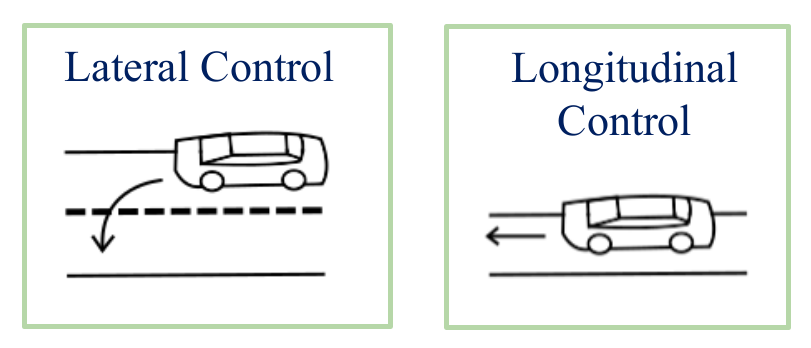
\includegraphics[scale=0.280]{img/intro_self_driving/lateral_longitu_control.jpeg}
\end{center}
\caption{Schematics of lateral and longitudinal motion.}
\label{lateral_longitu_control}
\end{figure}










\begin{figure}[!htb]
\begin{center}
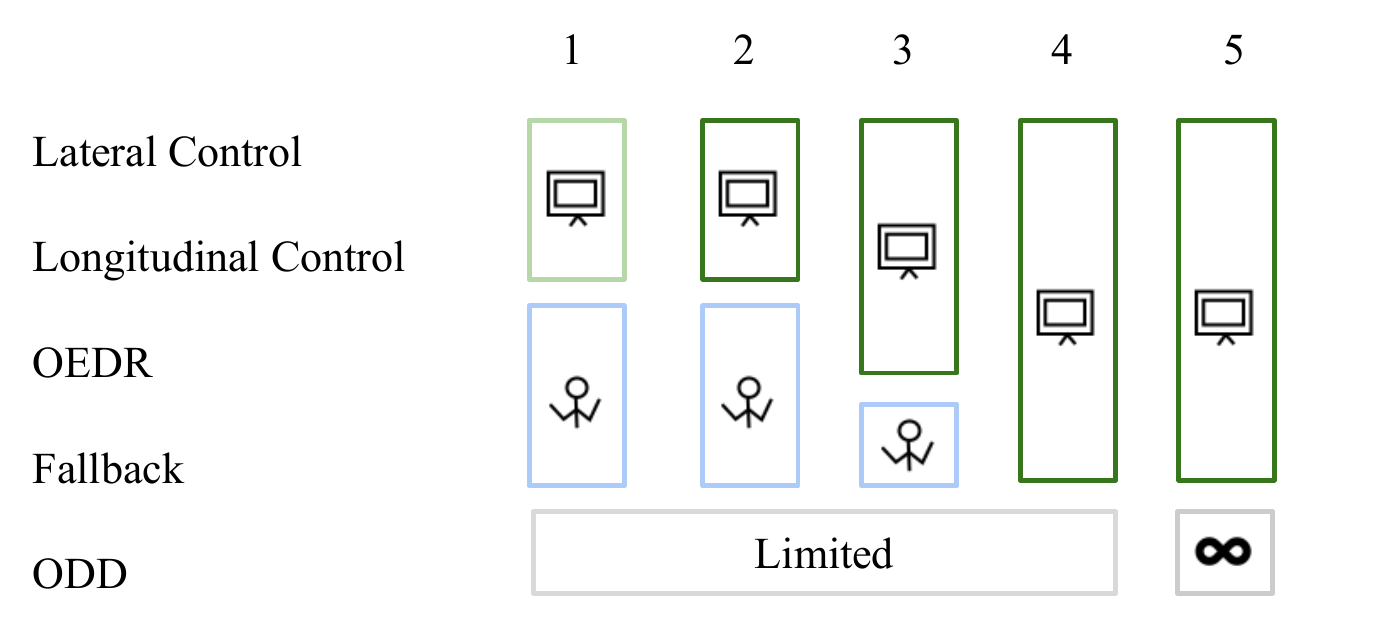
\includegraphics[scale=0.280]{img/intro_self_driving/levels_of_automation.jpeg}
\end{center}
\caption{Levels of automation.}
\label{levels_of_automation}
\end{figure}

\begin{framed}
\theoremstyle{remark}
\begin{remark}{\textbf{Primary actors in driving}}

There are three primary actors in driving: 

\begin{enumerate}
\item The (human) user
\item The driving automation system
\item Other vehicle systems and components.
\end{enumerate}
\end{remark}
\end{framed}


\subsection{Questions}
\label{introduction_self_driving_cars_questions}

\begin{enumerate}

\item Which of the following are components of longitudinal control? (Select all that apply)
\begin{enumerate}
\item Braking
\item Steering
\item Accelerating
\item Planning
\end{enumerate}

\item Which of the following is not an example of OEDR?

\begin{enumerate}
\item Stopping at red light
\item Finding a route from your location to a goal location
\item Slowing down when seeing a construction zone ahead
\item Pulling over upon hearing sirens.
\end{enumerate}

\item Which of the following tasks would you expect a Level 2 system to perform? (Select all that apply)

\begin{enumerate}
\item Maintain constant speed
\item Change lanes
\item Stay within a lane
\item Swerve and slow down to avoid a pedestrian
\end{enumerate}

\item What is the distinction between Level 3 autonomy and Level 4 autonomy? 


\begin{enumerate}
\item Level 3 systems only have lateral or longitudinal control. Level 4 systems have both.
\item Level 3 systems cannot drive on highways. Level 4 systems can.
\item Level 3 systems cannot perform OEDR. Level 4 systems can.
\item Level 3 systems require full user alertness. Level 4 systems do not.
\end{enumerate}

\item What distinguishes Level 5 Autonomy from Level 4?


\begin{enumerate}
\item Level 5 autonomy can operate on any weather condition. Level 4 cannot.
\item Level 5 autonomy has OEDR capability. Level 4 has not.
\item Level 4 has restricted operational design domain. Level 5 is unrestricted.
\item Level 5 autonomy can operate on any road surface and road type. Level 4 cannot.
\end{enumerate}

\end{enumerate}


\section{Perception}
\label{perception}
In the previous section, we learned how to classify automation according to its capabilities and operational design domain. 
In this section, we will start analyzing how a driving task is performed. Specifically, we will go over the many processes of perception. 
We will first define the perception task, listing out the requirements for perceptions such as what static and dynamic objects we need to identify, 
and what needs we have for tracking the ego vehicles motion through the environment. 
Finally, we will conclude with a discussion on some challenges to robust perception. So let's get started.


Very roughly speaking, any driving tasks can be broken down into two components, figure \ref{driving_task}. 

\begin{figure}[!htb]
\begin{center}
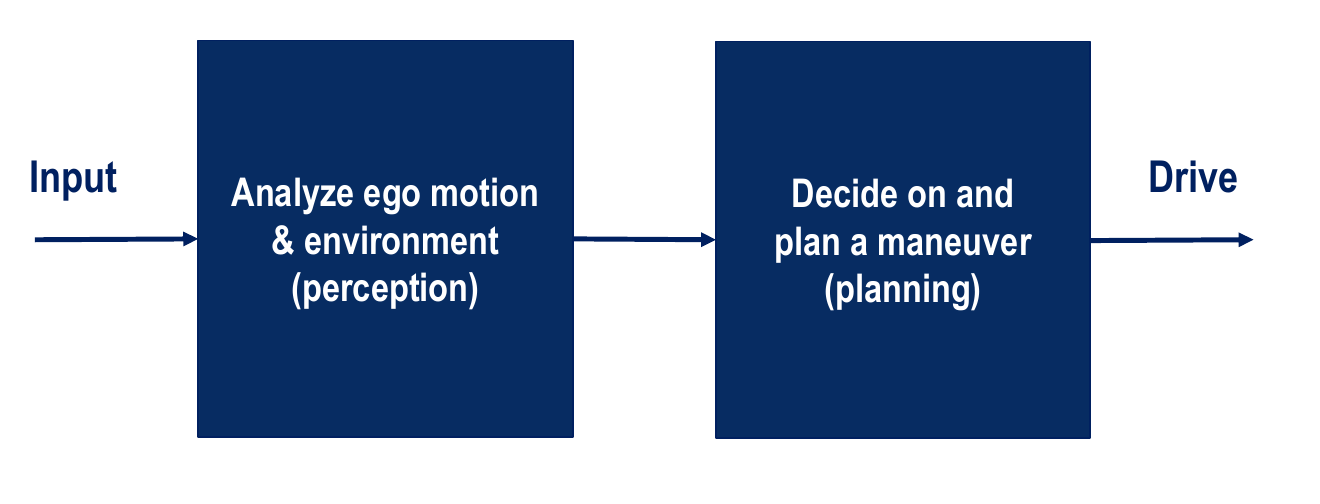
\includegraphics[scale=0.280]{img/intro_self_driving/driving_task.jpeg}
\end{center}
\caption{Schematics of the driving task as I/O process.}
\label{driving_task}
\end{figure}

First, we need to understand what's happening around us and where we are. So, we need to perceive our surroundings. 
Secondly, we need to make a driving decision. For example, should we accelerate or stop before a pedestrian about to enter the roadway? 
Recall from the previous section the concept of OEDR or object and event detection and response. 
Any driving task requires some kind of OEDR, that is, we need some way of identifying objects around us, recognizing events happening near us, and then responding to it. 
Recall that the classification of automated systems that we discussed had OEDR as one of the criteria. 
In other words, if we want to build a self-driving car, we need to be able to perform OEDR. Let's go further and analyze a crucial part of OEDR perception. 

\subsection{What is perception?}
So, what is perception? As we discussed, we want to be able to make sense of the environment around us and the way we're moving within it. 
In particular, for any agent or element on the road, we need to first identify what it is; a car, a cyclist, a bus, etc. 
On a second stage, we want to understand its motion; has it been moving in a certain way that can tell us what it will do next. 
As humans, we're really good at understanding patterns. 
However, it's still difficult for computer systems to be able to recognize these same patterns around us as quickly as we do. 
We can point to a car going straight and say, "Oh, it will be in this position in some amount of time in the future." 
This is what makes driving possible for us. So, this ability of predicting the trajectory of a moving object is really important to perception. 
If we can do this prediction correctly, we can make informed decisions. For example, if I know what the car in front of me is going to do next, 
then I can decide what to do next in such a way that both of our goals are met. 

Let's discuss the various elements we need to be able to identify for the perception task. 
First, we need to identify static elements. These are elements like roads and lane markings, things that segregate regions on the roads like zebra crossings, 
and important messages such as school up ahead. These are all on the road area, see figure \ref{static_objects}.

\begin{figure}[!htb]
\begin{center}
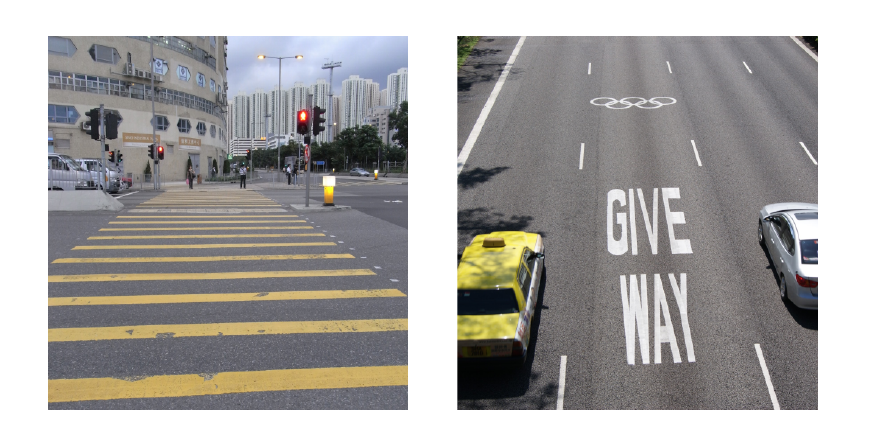
\includegraphics[scale=0.280]{img/intro_self_driving/static_objects.jpeg}
\end{center}
\caption{Lane markings and zebra crossings.}
\label{static_objects}
\end{figure}

Then there are off-road elements like curbs that define the boundaries within which we can drive. 

\begin{figure}[!htb]
\begin{center}
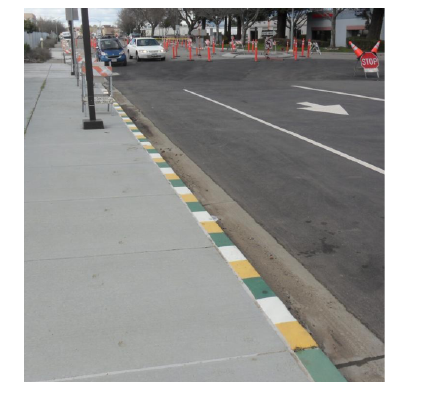
\includegraphics[scale=0.280]{img/intro_self_driving/static_objects_2.jpeg}
\end{center}
\caption{Off road signals.}
\label{static_objects_2}
\end{figure}

There are the on-road traffic signals that periodically change and signal whether you are allowed to move forward, or left, or right, or just stay stopped. 
Then there are all kinds of road signs like those telling you the speed limit, indicating direction, whether there is a hospital coming up, or a school coming up, and so on. 

\begin{figure}[!htb]
\begin{center}
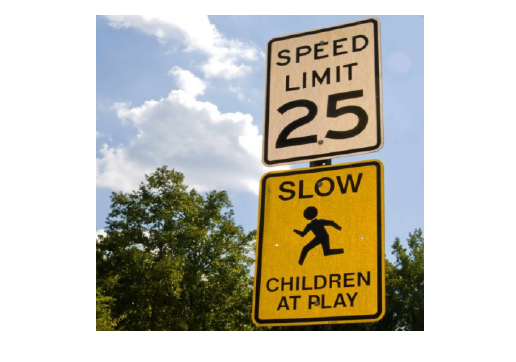
\includegraphics[scale=0.280]{img/intro_self_driving/road_signs.jpeg}
\end{center}
\caption{Road signs.}
\label{road_signs}
\end{figure}

Again, these are off-road elements. Finally, there are road obstructions. So, the orange cones that tell you construction is happening or that there is roadblock edge and so on, see figure \ref{construction_signs}. Also, these are on road elements. 


\begin{figure}[!htb]
\begin{center}
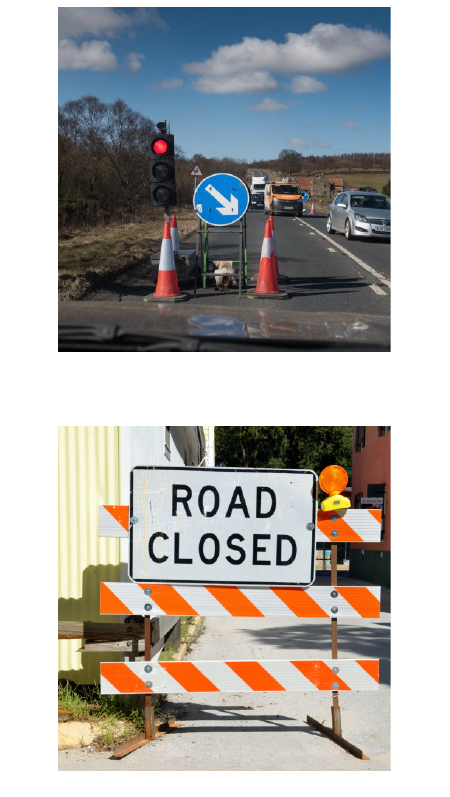
\includegraphics[scale=0.280]{img/intro_self_driving/construction_signs.jpeg}
\end{center}
\caption{Construction signs.}
\label{construction_signs}
\end{figure}

All the above can be classified as static elemens. Let's discuss the dynamic elements that we need to identify for perception. 
These are the elements whose motion we need to predict to make informed driving decisions. 
We need to identify other vehicles on the road, so four wheelers like trucks, buses, cars, and so on, and then we also need to identify and predict the motion of two wheelers, like motorcycles, bicycles, and so forth. These are all moving systems with more freedom than four wheelers, and so they are harder to predict. 
Finally, we should also be able to identify and predict the motion of pedestrians around us. 
How pedestrians behave is very different from vehicles as pedestrians are known to be much more erratic than vehicles in their motion because of the inherent freedom that humans have in the way they move. Another crucial goal for perception is ego localization. 
We need to be able to estimate where we are and how we are moving at any point in time. 
Knowing our position and how we are moving in the environment is crucial to making informed and safe driving decisions. 
The data used for ego motion estimation comes from GPS, IMU, and odometry sensors, and needs to be combined together to generate a coherent picture of our position. 
 

Now that we've discussed the main goals for perception, let's conclude this discussion by going over why perception is also a difficult problem. First, performing robust perception is a huge challenge. Detection and segmentation can be approached with modern machine learning methods, but there is much ongoing research to improve the reliability and performance to achieve human level capability. Access to large datasets is critical to this effort. 
With more training data, our segmentation and detection models perform better and more robustly, 
but collecting and labeling data for all possible vehicle types, weather conditions, and road surfaces is a very expensive and time-consuming process. 
Second, perception is not immune to censor uncertainty. There are many times that visibility can be challenging, or GPS measurements get corrupted, or LIDAR and Radar returns are noisy in terms of their position value. Every subsystem that relies on these sensors must take uncertain measurements into account. 
This is why it is absolutely crucial to design subsystems that can accommodate sensor uncertainty and corrupted measurements in every perception task. 
Then there are effects such as occlusion and reflection in camera or LIDAR data. 
These can confuse perception methods with ambiguous information that is challenging to resolve into accurate estimates of object locations. 
There are also effects such as drastic illumination changes and lens flare, or GPS outages and tunnels which makes some sensor data completely unusable or unavailable. 
Perception methods need multiple redundant sources of information to overcome sensor data loss. 
Finally, there's weather and precipitation that can adversely affect the quality of input data from sensors. 
So, it is crucial to have at least some sensors that are immune to different weather conditions, for example radar. 


\subsection{Questions}
\label{perception_questions}

\begin{enumerate}

\item Which of the following tasks are associated with perception? (Select all that apply) 
\begin{enumerate}
\item Estimating the motion of other vehicles
\item Identifying road signs
\item Responding to traffic light changes
\item Plannning routes on a map
\end{enumerate}

\item Which of the following can be on road objects? (Select all that apply) 

\begin{enumerate}
\item Potholes
\item Stop signs
\item Sidewalks
\item Vehicles
\end{enumerate}

\item Which of the following tasks pose challenges to perception? (Select all that apply) 

\begin{enumerate}
\item Having sensors work in adverse weather conditions
\item Having sensor occlusion and reflection
\item Handling sensor uncertainty
\item Detecting tracking and predicitng dynamic object motions
\end{enumerate}

\item Which of the following sensors are used for ego localization? (Select all that apply) 


\begin{enumerate}
\item Global Navigation Satellite System GNSS
\item Radar
\item Barometers
\item Inertial Measurement Unit (IMU)
\end{enumerate}

\item Which of the following objects would be relevant for perception in adaptive cruise control?


\begin{enumerate}
\item Road signs
\item Traffic lights
\item Other vehicles
\item Lane markings
\end{enumerate}

\end{enumerate}


\section{Driving Decisions}
\label{driving_decisions}
In this section, we will be discussing decision-making in a self-driving car system. 
In the previous section, we discussed the concept of perception which forms the first step in performing a driving task. 
The other steps in driving include decision-making and then, finally, executing the decisions. 
In this section, we will categorize planning informally on the basis of the window of time over which the decision has to be made and discuss some examples. 
Then we will go over a simple intersection scenario and try to list out some of the various decisions needed to complete the driving task successfully. 
We will then categorize planning formaly based on the type of logic we use to make the decisions. 
So, is our logic made up of well-defined rules that react only to currently available information about the driving environment? 
Or is it also dependent on trajectory predictions of other agents? Let's get started. 


Making driving decisions falls under the bigger umbrella of planning. When we make driving decisions, we usually have three kinds of decisions to make. 

\begin{itemize}
\item Long-term planning decisions. A question such as, how do I navigate from New York to Los Angeles or from my home to work? By answering this question, we have a mission plan, a high-level plan for the entire driving task. Mapping applications that you use today are able to give you these driving instructions: which roads to take, which lanes to be in, and so on. But driving needs much more than that. 
\item Short-term driving decision with questions like, is it safe to change lanes now? Or when should I execute a left turn at an intersection? 
\item immediate decisions or reactions. These decisions involve control and trajectory planning and answer questions like, how do I follow my lane on this curved road? 
What steering input should I apply? Should I accelerate or brake? If so, by how much.
\end{itemize} 


\subsection{Intersection Scenario}

Let's discuss a very simple example of a driving task and try to think about what kind of decisions are involved. Suppose you are approaching an intersection on your way home. 
The long-term planning stage requires you to turn left at this intersection. 
Now, let's look at the intermediate and short-term decisions that need to be made. 
First, let's assume that the intersection is controlled. 
That is, it has traffic lights. Since you are turning left, you have to identify if you need to make a lane change into a left turning lane. 
Then, as you're approaching this intersection, you choose to slow down, and to do so smoothly so that the passengers don't experience discomfort. 
Nobody likes a jerky driver after all. You then come to a stop just before the stop line, before a pedestrian crossing. 
These decisions on lane changes and stopping locations are all short-term planning decisions. 
However, we also need to think and respond to situations that arise along the way. 
We still need object and event detection and response. 
What if a vehicle pulls into the turn lane in front of you? You would want to stop earlier to make room for the other vehicle. 
What if the stop lines weren't marked? You would have to approximately judge where the implied stop line is and stop before the pedestrian crossing. 
What if there were other vehicles behind you or even stalled in the intersection? 
How does the decision to execute a left turn change based on the many possible scenarios that can rapidly arise in normal driving? 
All of these decisions fall into the immediate decision category and requires safe reactions from the planning system. 
The end result is an exploding list of possible decisions to evaluate on different timescales, even for a simple left turn scenario. 
This amounts to talking about different cases for the same intersection crossing or scenarios. 
In each scenario, we need a consistent set of choices to be evaluated in real time and updated as new information about the scene becomes available. 
Furthermore, because decisions to change lanes affect where to drive and which cars to regulate our position relative to, 
even a seemingly simple driving scenario requires three or four levels of decisions, and must then still be executed with careful vehicle control. 
This example is really only scratching the surface of the constant stream of decisions needed for motion planning. 
The bottom line is, driving is complicated. Let's go ahead and discuss a possible structure to represent these decisions in software. 


{\textbf{Reactive planning}}

One method to address the challenge of multilevel decision-making is reactive planning. 
In reactive planning, we define sets of rules that take into account the current state of the ego vehicle 
and other objects in the environment and produce immediate actions. 
So, these are rules that only consider the current state and not future predictions. 
Some examples of such rules would be, if there is a pedestrian on the road, stop. 
Or if the speed limit changes, adjust your speed to match it. 
In both of these rules, we just observe what is happening right now and make our decision based on immediately available information. 
But there are other kinds of planning as well. 

{\textbf{Predictive planning}}

In predictive planning, we make predictions on how other agents in the environment, like vehicles and pedestrians, will move over time. 
We use this current state and prediction information to define all of our decisions. 
Some examples of rules in predictive planning would be, that car has stopped for the last 10 seconds. 
It's probably going to stay stopped for the next few seconds. 
So, perhaps there is a way that I can move past it safely. 
Or a pedestrian is jaywalking. 
They will enter our lane by the time I get close to them. Let me slow down and give them a chance to cross the road ahead of me. 
As you can see, this is a more natural way to think, and relates closely to how humans operate vehicles. 
We predict where other objects on the road will be in the future before we make our decisions. 
This type of planning, however, relies on accurate predictions of the actions of the other 
actors in the environment, which adds a significant layer of complexity to the perception tasks. 
Nonetheless, predictive planning is the predominant method for self-driving cars, as it greatly expands the scenarios a vehicle can handle safely. 


Let's summarize this section. We discussed the planning problem and the different types of planning based on the window of time over which we have to act. 
These types are long-term, short-term, and immediate planning. 
Then we discussed a simple intersection scenario, where we had to make a left turn. 
We concluded that driving is a really hard problem since we have so many variables and possibilities that result. 
Then we discussed two different planning approaches: reactive planning and predictive planning. 
This is just the tip of the iceberg. There's clearly so much more we need to think about before making a decision during the driving task. 
 
Let's quickly recap what we learned this week. In this module, we explored the basic autonomous driving terminology that's useful for later weeks of the specialization. We then discussed the levels of automation, and came up with a taxonomy to characterize self-driving capabilities. Then we define the driving task and the major components of driving: perception, planning, and execution. We then listed the elements and agents in the environment we need to identify and track for perception. We also discussed why perception is so hard. Then we discussed planning with its different horizons, and looked at some decision-making approaches. In the next module, we will define the main components of self-driving cars, including both the hardware and software elements that make up a complete system. See you then.


\section{Review Questions}
\label{review_questions_chapter_1}

\begin{enumerate}

\item You’re at home and need to drive to work. During the trip, you will be performing OEDR tasks. Of the tasks below, which of the following is not an example of OEDR? 
\begin{enumerate}
\item Stopping at a red light
\item Slowing down when seeing a construction zone ahead
\item Maintaining a distance to a vehicle ahead
\item Pulling over upon hearing sirens
\end{enumerate}

\item Which of the following tasks are associated with perception? 

\begin{enumerate}
\item Identifying road signs
\item Respond to traffic lights
\item Planning routs on a map
\item Estimating the motion of other vehicles
\end{enumerate}

\item Before leaving, you decide to check the weather. The forecast states that over the next few days there will be both sun and rain along with some fog. Assuming your vehicle exhibits Level 5 autonomy, which of the following weather conditions can your vehicle operate

\begin{enumerate}
\item Clear and sunny
\item Windy heavy rainfall
\item Heavy fog
\item Light rainfall
\item all of the above
\end{enumerate}

\item You enter your autonomous vehicle and it drives your usual route to work. While the vehicle is driving, you decide to take a nap. For which levels of autonomy is this safe? (Select all that apply) 


\begin{enumerate}
\item 1
\item 2
\item 3
\item 4
\item 5
\end{enumerate}

\item You’re approaching an all ways stop sign and you want to make a right turn. Your vehicle is denoted in orange. There are 2 pedestrians currently crossing and another vehicle (denoted in green) approaching the stop sign from the left

\begin{figure}[!htb]
\begin{center}
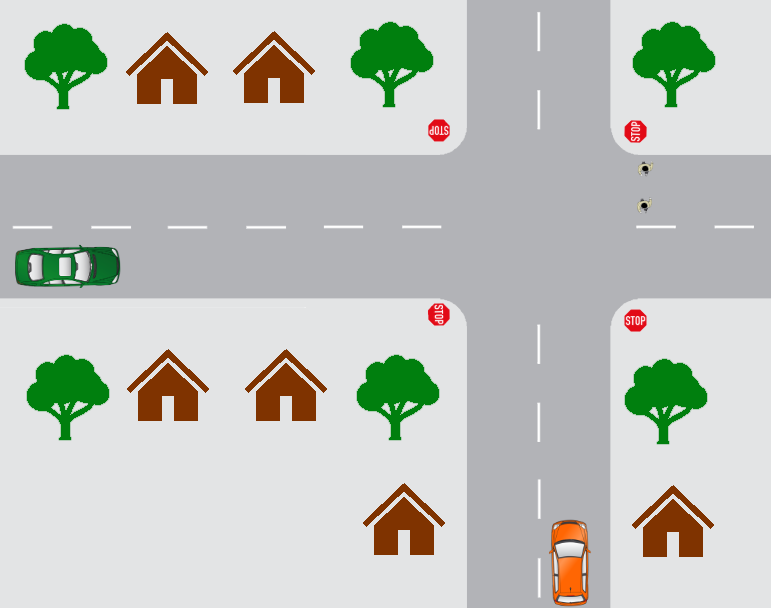
\includegraphics[scale=0.280]{img/intro_self_driving/summary_question_scenario_2.png}
\end{center}
\label{summary_question_scenario_2}
\end{figure}

This task involves multiple considerations, which of them are predictive planning? Select all that apply

\begin{enumerate}
\item At a stop sign, stop and look both ways before proceeding
\item Gradually decelerate while reaching the stop sign
\item The green car arrives at the stop sign after you and plans to travel straight through the intersection. 
You choose to move first
\item Wait for the pedestrians to finish crossing before turning
\end{enumerate}


\item Here are some rules for driving at a stop sign. 


\begin{itemize}
\item A) For non all-way stop signs, stop at a point where you can see oncoming traffic without blocking the intersection
\item B) If there are pedestrians crossing, stop until they have crossed
\item C) If you reach a stop sign before another vehicle, you should move first if safe
\end{itemize}

Which of the following is an appropriate priority ranking?

\begin{enumerate}
\item A, B, C
\item C, B, A
\item B, A, C
\item C, A, B
\item A, C, B
\end{enumerate}

\item Which of the following are off-road objects? (Select all that apply) 

\begin{enumerate}
\item Stop signs
\item Pedestrians
\item Curbs
\item Road markings
\item Trees
\end{enumerate} 

\item Suppose your vehicle has lane keeping assistance, which of these objects are relevant for its performance? (Select all that apply)

\begin{enumerate}
\item Stop signs
\item Pedestrians
\item Road markings
\item Trees
\item Curbs
\end{enumerate}

\item Which of the following sensors are used for the lane keeping assistance? (Select all that apply)

\begin{enumerate}
\item IMU
\item GPS
\item LIDAR
\item Barometers
\item Cameras
\end{enumerate}

\item You are on the highway and you see a truck in front of you. Assume the car is driving on the right-hand side of the road. 
There is also a blue car beside the truck in the other lane.


\begin{figure}[!htb]
\begin{center}
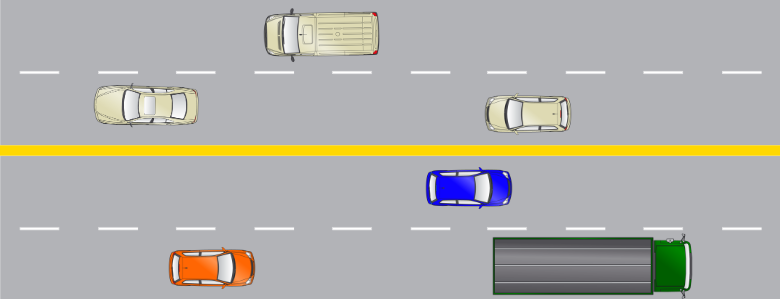
\includegraphics[scale=0.280]{img/intro_self_driving/summary_question_scenario_3.png}
\end{center}
\label{summary_question_scenario_3}
\end{figure}

Your vehicle follows the truck and maintains a constant distance away. What kind of control is this?

\begin{enumerate}
\item Longitudinal
\item Fallback
\item OEDR
\item Lateral
\end{enumerate}

\item You decide to change lanes to pass a truck. What kind of decision is this?

\begin{enumerate}
\item Reactive
\item Rule-based planning
\item Short term planning
\item Long term planning
\item Immediate
\end{enumerate}

\item Which of the following tasks are rule-based planning? (Select all that apply) 

\begin{enumerate}
\item Doing a lane change, maintain our current speed or accelerate slightly
\item If there are vehicles directly beside us on the lane, it is unsafe to lane change
\item If the vehicle in front is going to slow down sharply, then avoid performing a lane change.
\end{enumerate}

\item  Suppose the blue vehicle in figure \ref{summary_question_scenario_3} suddenly brakes and you decide to abort the lane change. 
If your vehicle can respond automatically and remain in its own lane, what is the minimum level of autonomy of your vehicle?

\begin{enumerate}
\item 1
\item 2
\item 3
\item 4
\item 5
\end{enumerate}

\item The blue vehicle in figure \ref{summary_question_scenario_3} returns to normal speed and you can now safely change lanes. Your car is performing the lane change, what kind of control is this?

\begin{enumerate}
\item Longitudinal
\item Fallback
\item OEDR
\item Lateral
\end{enumerate}


\item You are almost at work but encounter a construction site. Assume the car is driving on the right-hand side of the road. 
Your vehicle is denoted in orange in  figure \ref{summary_question_scenario_4}.

\begin{figure}[!htb]
\begin{center}
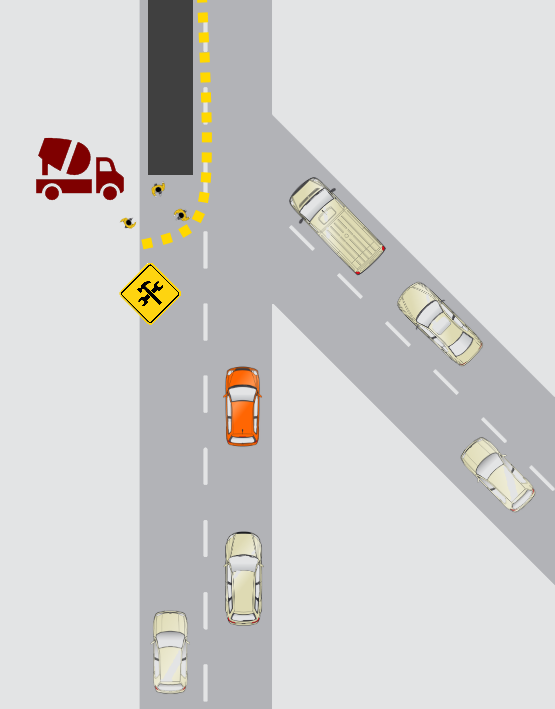
\includegraphics[scale=0.280]{img/intro_self_driving/summary_question_scenario_4.png}
\end{center}
\label{summary_question_scenario_4}
\end{figure}

You see a construction site where the workers are repaving a road full of potholes. They are using jackhammers which can cause dust clouds.
You create the  decision tree in figure \ref{summary_question_scenario_4_flowchart} for getting through the construction site. 
From the diagram, which of the following decisions should you make? (green is true, red is false) 

\begin{figure}[!htb]
\begin{center}
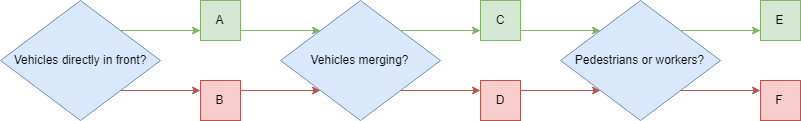
\includegraphics[scale=0.280]{img/intro_self_driving/summary_question_scenario_4_flowchart.png}
\end{center}
\label{summary_question_scenario_4_flowchart}
\end{figure}

\begin{enumerate}
\item A (True)
\item B (False)
\item C (True)
\item D (False)
\item E (True)
\item F (False)
\end{enumerate}

\item Here are a set of rules for making these decisions, arrange them in an appropriate prioritization

\begin{itemize}
\item If there are no vehicles ahead, accelerate to the speed limit
\item Drive slowly in construction zones
\item If there are pedestrians or workers directly ahead in the current lane, stop
\item Yield to merging vehicles, if necessary 
\end{itemize}

\begin{enumerate}
\item 1, 2, 3, 4
\item 2, 3, 4, 1
\item 3, 4, 1, 2
\item 3, 4, 2, 1
\end{enumerate}

\item  You’re finished work and need to drive back home, but it’s nighttime.
You plan a new path home on your GPS application to avoid the construction site, what type of planning is this?

\begin{enumerate}
\item Immediate
\item Long term planning
\item Reactive
\item Short term planning
\item Rule based planning
\end{enumerate}


\item Your new path goes through a school zone and you see the school zone sign. You decide to slow down despite there being no pedestrians or children (it’s nighttime). What sort of planning is this?

\begin{figure}[!htb]
\begin{center}
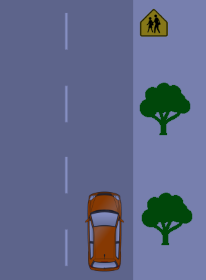
\includegraphics[scale=0.280]{img/intro_self_driving/summary_question_scenario_5.png}
\end{center}
\label{summary_question_scenario_5}
\end{figure}

\begin{enumerate}
\item Short term planning
\item Immediate planning
\item Long term planning
\item Rule based planning
\item Reactive planning
\end{enumerate}

\end{enumerate}
